\subsection{Giao diện thông báo của người dùng}

\begin{figure}[H]
    \centering
    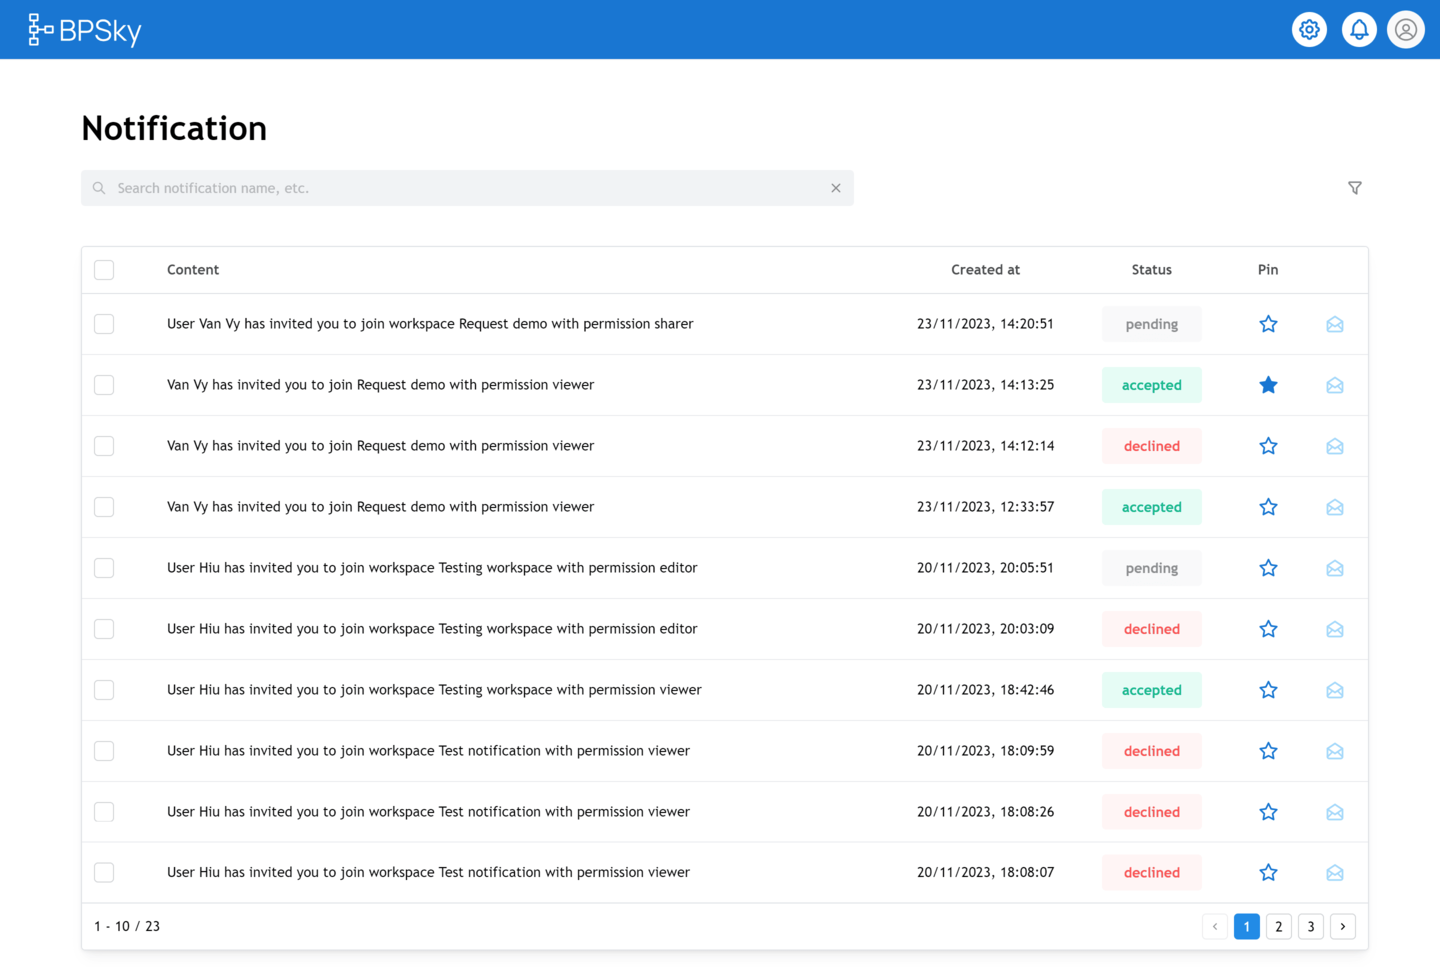
\includegraphics[ width = \linewidth]{Content/Hiện thực hệ thống/documents/Hiện thực giao diện người dùng/images/NotificationPage.png}
    \vspace{0.5cm}
    \caption{Giao diện trang thông báo của người dùng}
    \label{fig: Giao diện trang thông báo của người dùng}
\end{figure}

Người dùng có thể truy cập vào trang thông báo bằng cách chọn icon hình chuông ở phía trên thanh điều hướng. Tại đây, người dùng có thể xem danh sách những thông báo mà hệ thống gửi tới người dùng. Mỗi item thông báo sẽ tùy thuộc vào loại thông báo tương ứng mà hiển thị trạng thái khác nhau (bao gồm "Approved" - chấp nhận, "Declined" - từ chối, "Pending" - đang chờ phản hồi). Người dùng có thể đánh dấu thông báo quan trọng bằng cách nhấn vào icon ngôi sao ở mỗi item thông báo, thông báo quan trọng có thể được lọc thông qua công cụ filter.